% Refinement via Arc-Length Deficit
\section{Refinement via Arc-Length Deficit}
Mentioned above, a way of determining ``how well'' a discretization approximates a curve was to consider the difference between arc lengths.  This posed another way as ``how well'' it captures curvature.  Locally, it is important for each segment in the discretization to represent the local geometry present in the curve.  If a segment is to be subdivided in order to improve the discretization, then it should be subdivided in a way that is most effective/efficient locally.  Also, if the purpose of the refinement process is to minimize the actual arc length minus the discrete arc length, then an optimization problem can be formed where an objective function is minimized as the combined length of the segments in the discretization approach that of the curve.

Let $C(u)$ be a parameterized curve, and $D$ be a discretization of the curve comprised of a number, $n_t$, of points, $P_i : i \in \{1,...n_t\}$, and segmenets, $S_j : j \in \{1,...,(n_t-1)\}$. Segment $S_j$ is defined by two successive parameterization values, $u_j$ and $u_{j+1}$. If $L(S)$ is a function that calculates the length of a segment  in $(x,y,z)$ space then the optimization problem can be stated as:
\begin{equation}
\begin{aligned}
& \underset{u_i}{\text{minimize}}
&& O=-\sum{_{j=2}^{n_t-1}L_j} \\
& \text{subject to}
&& (u_1 = a, u_1<u_2, u_2<u_3,..., u_{n_t-2}< u_{n_t-1}, u_{n_t} = b)
\end{aligned}
\end{equation}

\noindent The resulting optimization problem is linear[PROVE] and a variety of standard methods (subsets of linear programming) could be used to obtain a solution.  The analysis and calculation are straightforward for a defined number of interior points.  For this method to be practical, however, one would have to know a priori how many points on the interior of the curve were desired.  Either that, or repeatedly solve the optimization problem with an increasing number of interior points until the combined length of the segments in the discretization converged to a desirable tolerance.

One could not formally include the number of interior points into the definition of the optimization problem because the number of interior points could only be given a lower bound, 0.  An upper bound is needed due to the fact that the (not an) ``optimal'' discretization (as defined above) without an upper bound contains an infinite amount of interior points.  In order to impose an upper bound, one could constrain the problem further with a lower bound on the distance between points:

a user-defined minimum tolerance, $e$, is easily worked into the set of constraints, where $P_i$ represents a point in non-parametrized, $(x,y,z)$, space: \\
$(P_1 = \alpha, P_1+e <= P_2, P_2+e <= P_3, … , P_{n_t-2}+ e <= P_{n_t-1}, P_{n_t} = \beta)$ \\

\noindent An upper bound on the distance between points could also be implemented, where $P_i$ represents a point in non-parameterized, $(x,y,z)$, space:

a user-defined maximum tolerance, $m$, is easily worked in as an additional set of constraints: \\
$(P_1 = \alpha, P_1+m >= P_2, P_2+m >= P_3, … , P_{n_t-2}+ m >= P_{n_t-1}, P_{n_t} = \beta)$ \\

\noindent The definition of a lower and upper bounds for the distance between points implicitly defines an upper and lower bound for the number of interior points.  The implicit definition would be in the form of an over-constrained problem where solutions did not exist for too many or too few points.  For instance, too many points could not satisfy the minimum-distance set of constraints and too few points could not satisfy the maximum-distance set of constraints.  However, explicitly determining these bounds for $n_t$ would prove difficult.  It could, for example, involve repeatedly sampling the curve to determine the maximum number of e-length segments and the minimum number of m-length segments.  This would be possible, but inefficient.  Another option is to estimate the number of points needed \cite{cuilliere97}.  However, if $n_t$ is to be estimated then the discretization is not guaranteed to optimal. Therefore, the conclusion is that a global optimization problem, while possible, is not very practical in this case.  One of the aims of this work is to accelerate the generation of suitable grids for simulation; and moving the bottleneck for grid generation to the lowest level in the grid generation hierarchy just increases the amount of time required to generate a grid.  The above method does however represents a solution to the problem of generating automated, optimal edge-grids.

Others have attempted dynamic programming methods for generating ``optimal'' discretizations for digital curves \cite{horng02}.  However, in general this should prove no more effective than any of the approaches mentioned above.  It is true that the problem of generating a discretization to accurately represent a curve exhibits optimal substructure—which is defined where ``...an optimal solution can be constructed efficiently from optimal solutions to its subproblems.'' \cite{cormen01}  However, the number of distinct subproblems available that represent an optimal solution at a defined error bound can be infinite.  Therefore, instead of trying to find an optimal number of nodes required for an optimal discretization (which seems very inefficient), the proposed algorithm will use a divide-and-conquer (recursive) approach to generating an ideal discretization relative to a given tolerance.  The combination of the optimized segments represents an optimal discretization for the entire curve.

This would generate an optimal solution using two segments to represent the entire curve—which can be stated another way as maximizing the perimeter of the triangle formed by the existing segment and the two new segments.  Consider that the red triangle in Figure-\ref{CurvatureRatioTriangles} has a larger perimeter than the blue triangle; therefore the red triangle would be considered ``more optimal.'' The above optimization problem could then be applied recursively to each new segment with $n_t=3$.  This process breaks the task of optimizing a discretization for an entire curve into optimizing a simple discretization for smaller section of the curve with the following algorithm.  The optimization algorithm described above with $n_t=3$ for a given segment is:

\begin{algorithm}
\caption{Optimization Algorithm with $n_t=3$}\label{localoptimize}
\begin{algorithmic}[1]
\State $n_t = 3$
\State $u_i : i \in \{1,2,3\}$
\State $u_1 $ and $u_3$ define the segment $S_{1,3}$
\Procedure{Local Optimization}{$S_{1,3}$}
  \State $L(S_{1,3}) =\textnormal{ length of segment}$
  \State Place interior point $u_2$ to maximize $L(S_{1,2})+L(S_{1,3})$ within $tolerance$
\EndProcedure
\end{algorithmic}
\end{algorithm}

The would be applied for each segment in the discretization by:

\begin{algorithm}
\caption{Optimization Algorithm for Discretization}
\begin{algorithmic}
  \State $D(S_j) : j \in {1}$
  \State push $S_1$ into $list$ \Comment{$list$ is $queue$ if breadth-first, $stack$ if depth-first}
  \While{$list$ is not empty}
    \State pop $S_j$ from $list$
    \If {$S_i$ is optimal}
      \State do nothing
    \Else
      \State optimize $S_j$ with Algorithm: \ref{localoptimize}
      \State push $S_{i,i+\frac{1}{2}}$ into $list$
      \State push $S_{i+\frac{1}{2},i+1}$ into $list$
    \EndIf
  \EndWhile
\end{algorithmic}
\end{algorithm}

The above algorithm is straightforward and is often referred to as adaptive refinement or enrichment (see above).  Also, since the discretization of the curve exhibits optimal substructure, the starting point to the optimization algorithm and the method of refinement or enrichment are irrelevant to the extent to which they prevent an optimal solution from being generated.  However, the initial discretization and choice of refinement strategy/order of application obviously con
tributes to the efficiency of the algorithm.

Now to define the optimization part of the above algorithm:  Divide and conquer can be considered to be based on multi-branched recursion.  The objects to be constructed at the end of the recursion are the smallest set of segments that approximates the arc-length of the curve to a defined precision.  This is not quantifiable without the a priori knowledge of the arc-length of the curve.  As discussed above, calculating the length of a curve for this application is impractical.  So how can the ``goodness'' of a discretization be measured?  At each step, the discretization will be refined on each segment by locally optimizing an objective function analogous to the one developed above.  In order to minimize each segment’s objective function, arc length deficit ($ALD$), then a point $P$ has to be placed on the curve between the segment such that the new sum of the arc lengths is changed maximally.  Since this entire project is to be done without calculating derivatives (see reasons above), the optimization scheme chosen here is not given access to derivative information either.  Since the optimization function is a non-negative planar curve, $(O: C \rightarrow ALD)$, any line-searching method of optimization could be used.  However, the method cannot have any requirements on differentiability due to the possibility that the derivative of $O$ could be discontinuous if the curve passed through the segment.  Consider the function $f(x)=x^3-3x^2-144x+432$, plotted in red in Figure-\ref{OptimizationFunctionExample} with the blue line representing the corresponding segment.  The middle figure shows the graph of the optimization function (as defined above).  Notice at the root, 3, the curve crosses the x-axis and the derivative of the optimization function does not exist.  This can be seen right Figure-\ref{OptimizationFunctionExample} which is a plot of the derivative of the optimization curve.  The red line represents the limit approaching from $-\infty$ and the blue line represents the limit approaching from $+\infty$.

\begin{figure}[h!]
  \center{
    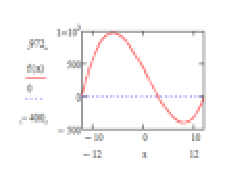
\includegraphics{Figures/CurvePlot.eps}
    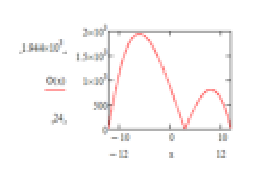
\includegraphics{Figures/OFunctionPlot.eps}
    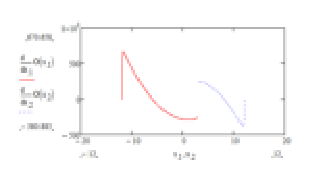
\includegraphics{Figures/ODerivativePlot.eps}
  }
  \caption{\label{OptimizationFunctionExample} Caption}
\end{figure}

The Golden-Section Search Method is implemented here since it meets all of the above criteria and has the possibility to converge superlinearly \cite{brent73}--unlike the bisection method.  If the length of each segment locally approaches the portion of the curve it represents (local objective function is minimized), then the global length of the discretization approaches the global length of the curve (a restatement of the property of optimal substructure).  Also, since the optimization algorithm for each segment is only concerned about the portion of the curve it represents, then this method exhibits scale-independence—which was one of the requirements for the algorithm.

Recursive algorithms require stopping criteria.  In this case the stopping criteria should not permit the method to infinitely subdivide the curve.  For instance, the aforementioned minimum and maximum segment lengths can be used (and were implemented here).  Even though using a minimum edge length would prevent the infinite subdivision of the curve, another criteria is needed such that the minimum segment length is not needed to satisfy the criteria.  This stopping criterion could be in the form of a delta-segment length.  That is, if the new segments’ combined length is below a defined fraction larger than the existing segment then it should not be subdivided.  This is a ``pure-greedy'' method of subdivision, in that it does not consider the rest of the ``solution'' when deciding to stop.  One problem with this set of stopping criterion is immediately apparent: the ``large'' segments could potentially not be subdivided because locally it is not justified—even if the subdivision of that large segment would cause a global change in the length of the curve that is significant.  This value, global delta-segment, would have to be smaller than the one used locally for each segment; otherwise it would have no effect.  Therefore, an additional criterion is needed to determine if a segment should be subdivided: if the total change in length of the discretization would be changed by a defined fraction then it should be subdivided.  The addition of this last subdivision criterion makes the method ``less-greedy''.  This set, minimum segment length, maximum segment length, local delta-segment, and global delta-segment define a robust, minimum set of criterion needed for generating an optimum solution to the problem of representing a curve via arc-length deficit.

